\documentclass[11pt,italian]{article}
\usepackage[T1]{fontenc}
\usepackage[utf8]{inputenc} %utf8 % lettere accentate da tastiera
\usepackage[italian]{babel} % lingua del documento
\usepackage{blindtext}
\usepackage{enumitem}
\usepackage{float}
\usepackage{xcolor}   % for \textcolor
\usepackage{listings}
\lstset{
  basicstyle=\ttfamily,
  columns=fullflexible,
  frame=single,
  breaklines=true,
  postbreak=\mbox{\textcolor{red}{$\hookrightarrow$}\space},
}
\usepackage{hyperref}
\hypersetup{
    colorlinks = true,
    linkbordercolor = {white},
    urlcolor = blue
}
\usepackage{graphicx}
\graphicspath{ {./images/} }

% Italian syntax spacing
\frenchspacing

% Line height
\renewcommand{\baselinestretch}{1.15}

\title{
	Metodi del Calcolo Scientifico \\
	\normalsize Risoluzione di sistemi lineari tramite il metodo di Cholesky \\
}

\date{\small A.A. 2019/2020}

\author{
	\normalsize
	\textsc{Silva Edoardo} 816560 \\
	\normalsize
	\textsc{Zhigui Bryan} 816335 \\
	\normalsize
	\textsc{Marchetti Davide} 815990
}

\begin{document}

\maketitle

\section*{Abstract}
Lo scopo di questo progetto è di studiare l'implementazione del metodo di Choleski per la risoluzione sistemi lineari per matrici sparse, simmetriche e defite positive in ambienti di programmazione open source e di compararli con l'implementazione di MATLAB.

Il confronto avverrà in termini di tempo, accuratezza, impiego della memoria e anche facilità d'uso sia in ambiente Linux che Windows, eseguendo il codice su diverse matrici sparse derivate da problemi reali e raccolte nella \textbf{SuiteSparse Matrix Collection}.

\section{Analisi dell'implementazione}

\subsection{MATLAB}
Per la decomposizione di cholesky, MATLAB mette a disposizione il modulo \textbf{cholesky.matlab} contenente tutto il necessario. In particolare è stata utilizzata la funzione \textbf{chol}

\subsubsection*{Utilizzo}
\lstinline{R = chol(A, [triangle])}: Fattorizza la matrice $A$ simmetrica definita positiva in una matrice triangolare superiore $R$ tale che $A=R^{-1}R$.
Il parametro \lstinline{triangle} permette di scegliere se attuare la decomposizione in una matrice triangolare superiore (opzione di default) o traiangolare inferiore. In quest'ultimo caso, la matrice $R$ risultante dall'equazione soddisferà l'uguaglianza $A = RR^{-1}$.

\subsubsection*{Manutenzione}
La libreria è stata rilasciata per la prima volta nell'aggiornamento R2013a MATLAB. Attualmente, è ancora supportata e non presenta lacune o problemi che sono stati riscontrati durante il suo l'utilizzo.

\subsubsection*{Licenza}
Essendo MATLAB un software closed-source, non è possibile accedere al codice sorgente del modulo.

\subsection{Open-Source (C++)}
Dopo un'attenta analisi e comparazione di diverse opzioni, l'implementazione in C++ è stata costruita utilizzando \textbf{Eigen},  libreria che si pone l'obiettivo di essere leggera ed offire supporto alle operazioni su vettori e matrici dense e sparse.

\subsubsection*{Utilizzo}
\lstinline{Eigen::loadMarket(A, filename)}: Importa i valori di una matrice sparsa memorizzata in un file \lstinline{.mtx} nella matrice fornita come primo argomento. Nel nostro programma, \lstinline{A} è definita come \lstinline{Eigen::SparseMatrix<Type>}.

Il modulo \lstinline{unsupported/Eigen/SparseExtra} che contiene queste funzionalità è attualmente deprecato.

\begin{itemize}
\item \textbf{Eigen::VectorXd::Ones(A.rows()):} dichiara matrice di dimensioni fissate (prese dalle dimensioni della matrice A), package 'VectorXd' usato per le operazioni su matrici dinamiche di double.
	\item \textbf{Eigen::SimplicialCholesky<SpMat> chol(A):} Pacchetto creato per gestire matrici di grandi dimensioni con pochi elementi diversi da 0. Implementa uno schema di rappresentazione e gestione dei valori diversi da 0 con uso di poca memoria e alte prestazioni.\newline Il metodo chol(A) implementa la fattorizzazione di Cholesky della matrice A.
	\item \textbf{Eigen::VectorXd x\_ap = chol.solve(b):} Applicazione del risolutore iterativo per risolvere la fattorizzazione.
\end{itemize}

\subsubsection{Manutenzione}
Eigen è in sviluppo attivo, tuttavia, alcuni moduli sono marcati come deprecati e non ne è garantito il loro pieno funzionamento. Un esempio di questi è il modulo MarketIO, che permette di effettuare operazioni di Input e Ouput con file in formato Matrix Market (.mtx).

\subsubsection{Problemi}
Durante lo sviluppo, l'utilizzo di una classe deprecata ha inizialmente rallentato lo sviluppo. Infatti, delle matrici importate tramite \lstinline{MarketIO} veniva ignorato il fatto che fossero salvate come simmetriche o meno.

La soluzione a questo problema è stata messa in pratica modificando lo script matlab \lstinline{mmwrite} di conversione per file \lstinline{.mat} in \lstinline{.mtx} e rigenerando le matrici a partire dai file \lstinline{.mat}, assicurandosi che venissero salvati correttamente tutti gli elementi della matrice.

\subsubsection{Licenza}
Eigen è un software gratuito ed open-source rilasciato con licenza Mozilla Public License 2.0 (MPL2: simple weak copyleft license) dalla versione 3.1.1.

\section{Specifiche hardware}

\section{Risultati}

\subsection{Windows}
\subsubsection*{Tempo}
\begin{figure}[H]
	\makebox[\textwidth][c]{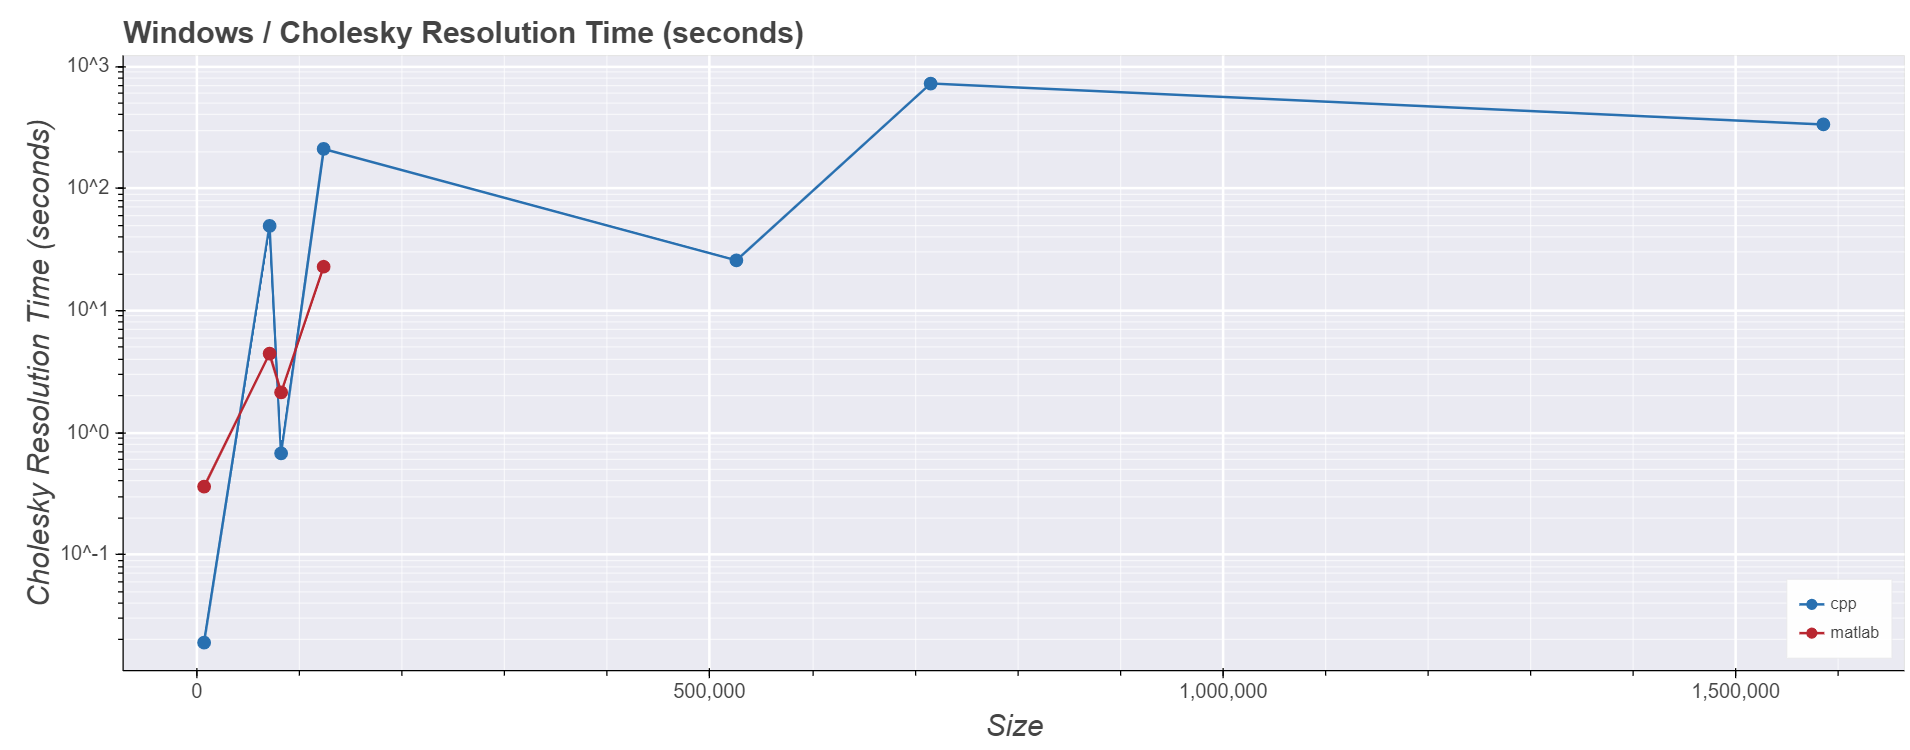
\includegraphics[width=1.4\linewidth]{windows_solve.png}}
\end{figure}

\subsubsection*{Errore relativo}
\begin{figure}[H]
	\makebox[\textwidth][c]{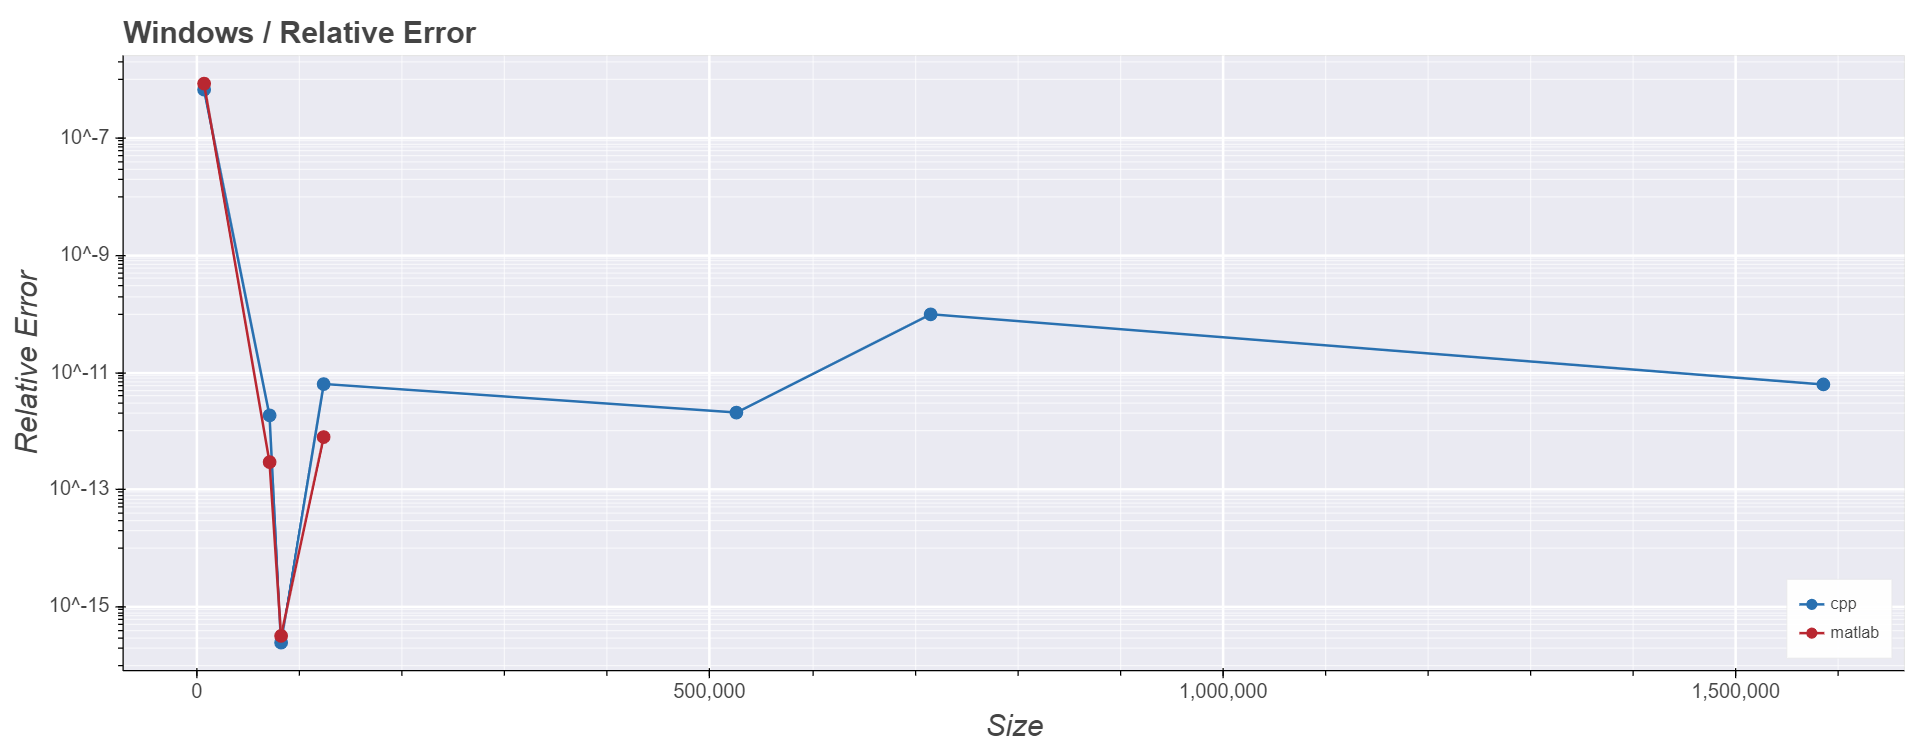
\includegraphics[width=1.4\linewidth]{windows_error.png}}
\end{figure}

\subsubsection*{Memoria}
\begin{figure}[H]
	\makebox[\textwidth][c]{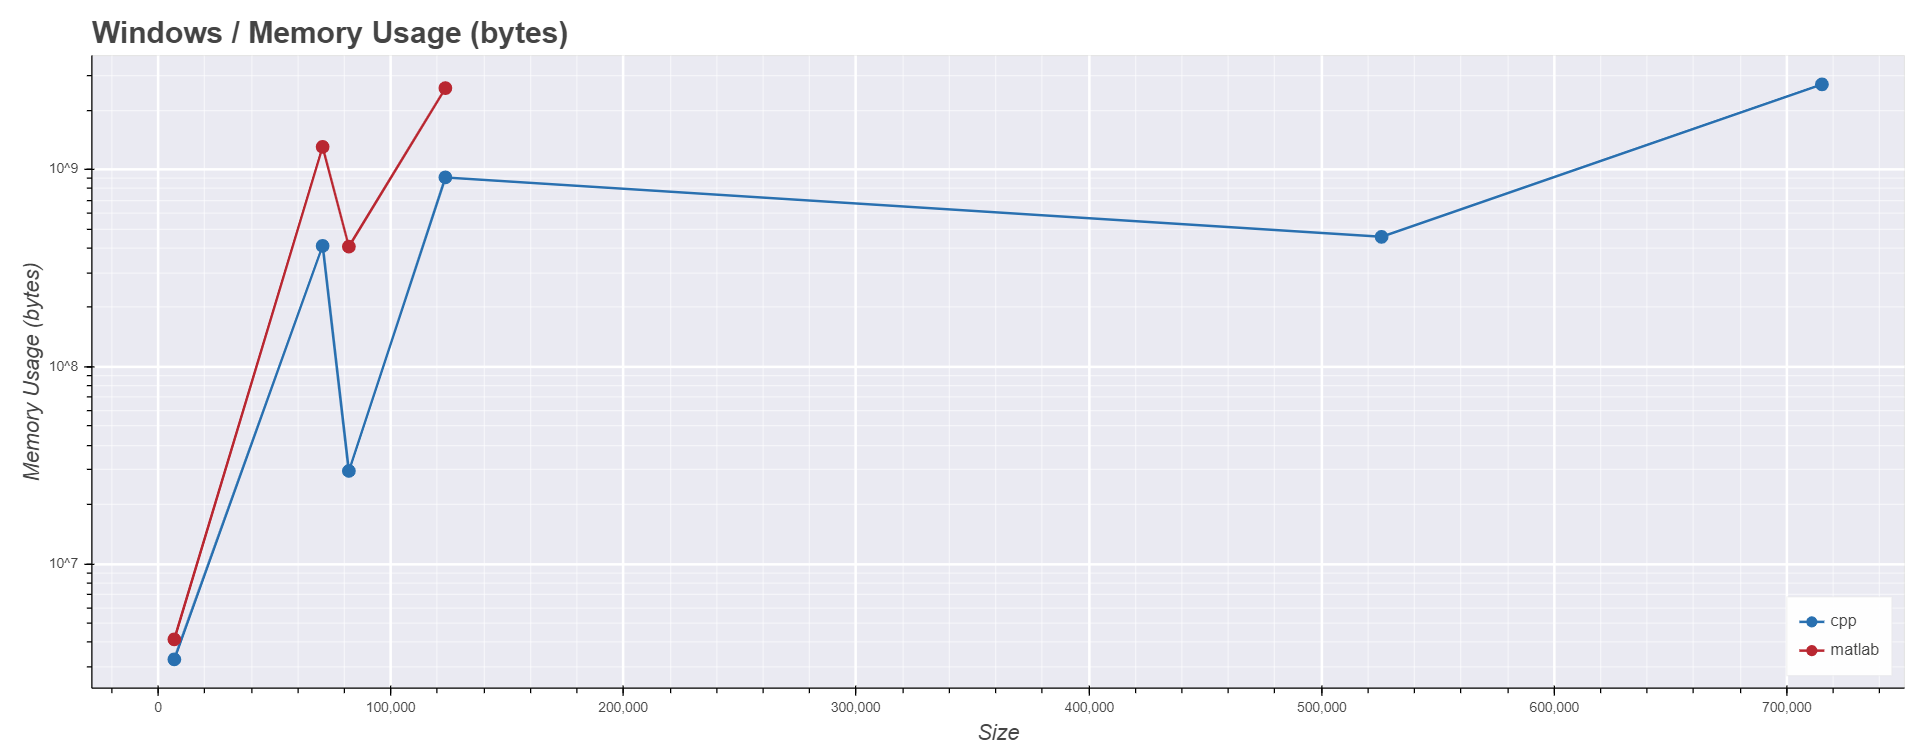
\includegraphics[width=1.4\linewidth]{windows_memory.png}}
\end{figure}

\subsection{Linux}
\subsubsection*{Tempo}
\begin{figure}[H]
	\makebox[\textwidth][c]{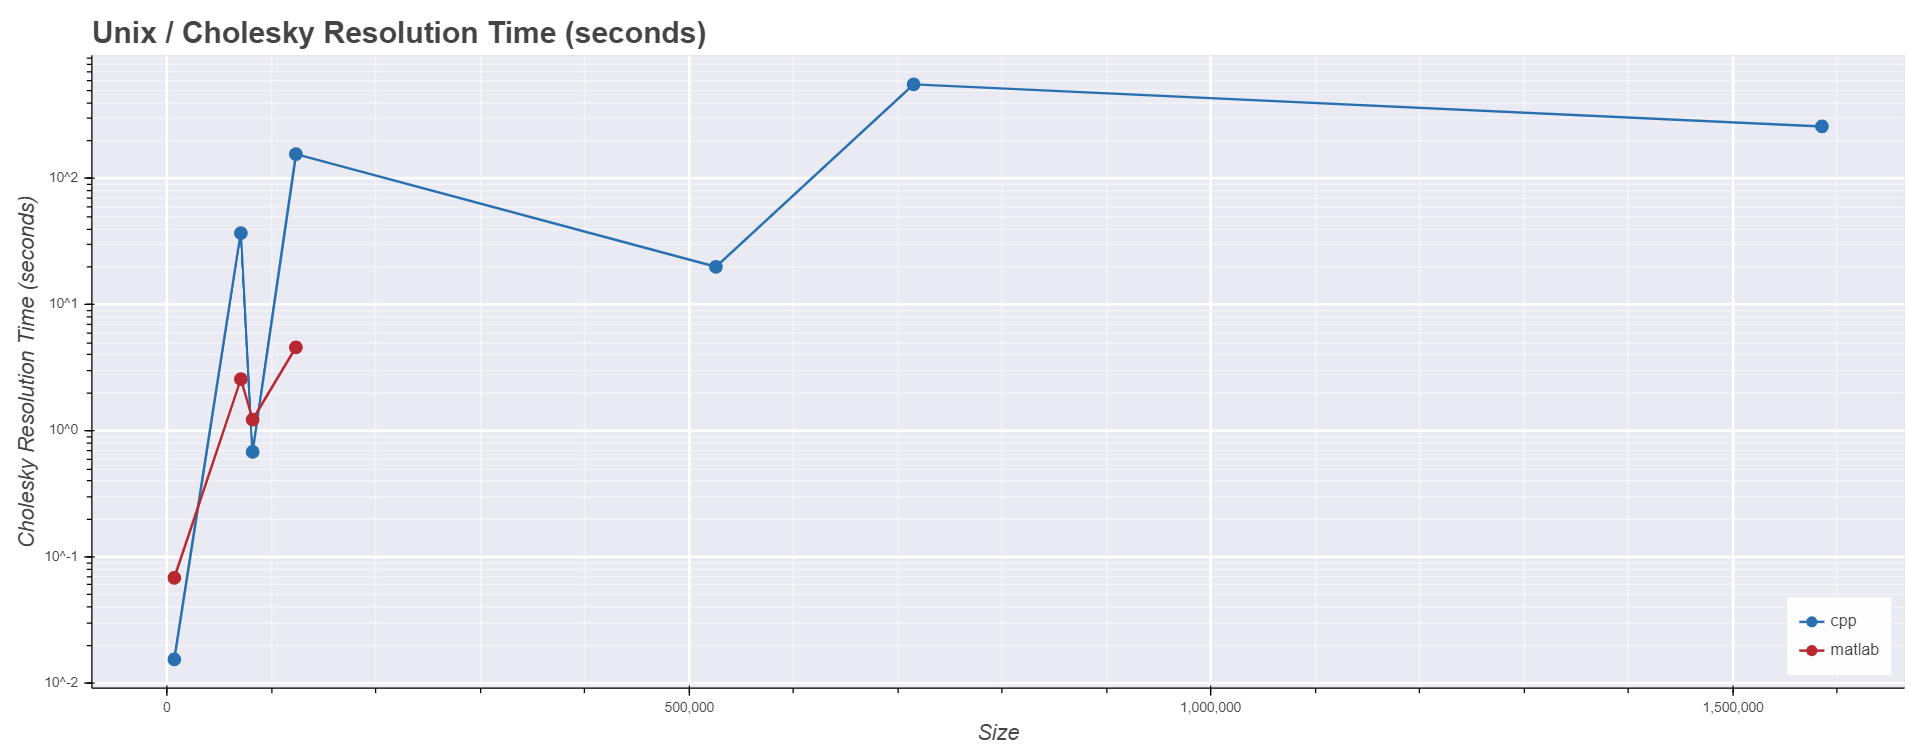
\includegraphics[width=1.4\linewidth]{unix_solve.png}}
\end{figure}

\subsubsection*{Errore relativo}
\begin{figure}[H]
	\makebox[\textwidth][c]{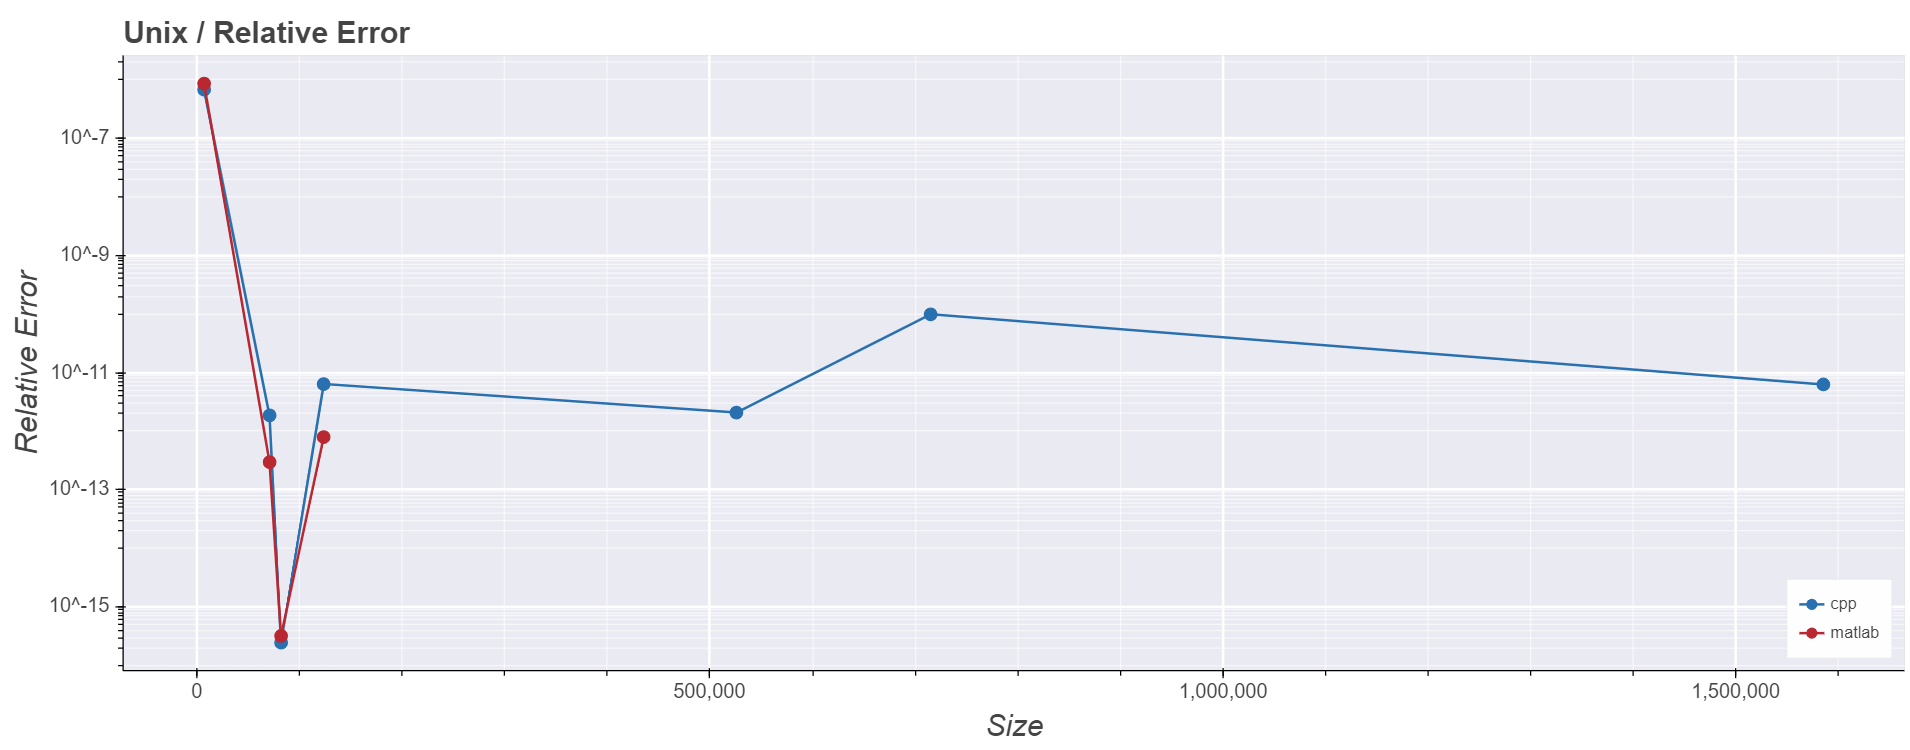
\includegraphics[width=1.4\linewidth]{unix_error.png}}
\end{figure}

\subsubsection*{Memoria}
\begin{figure}[H]
	\makebox[\textwidth][c]{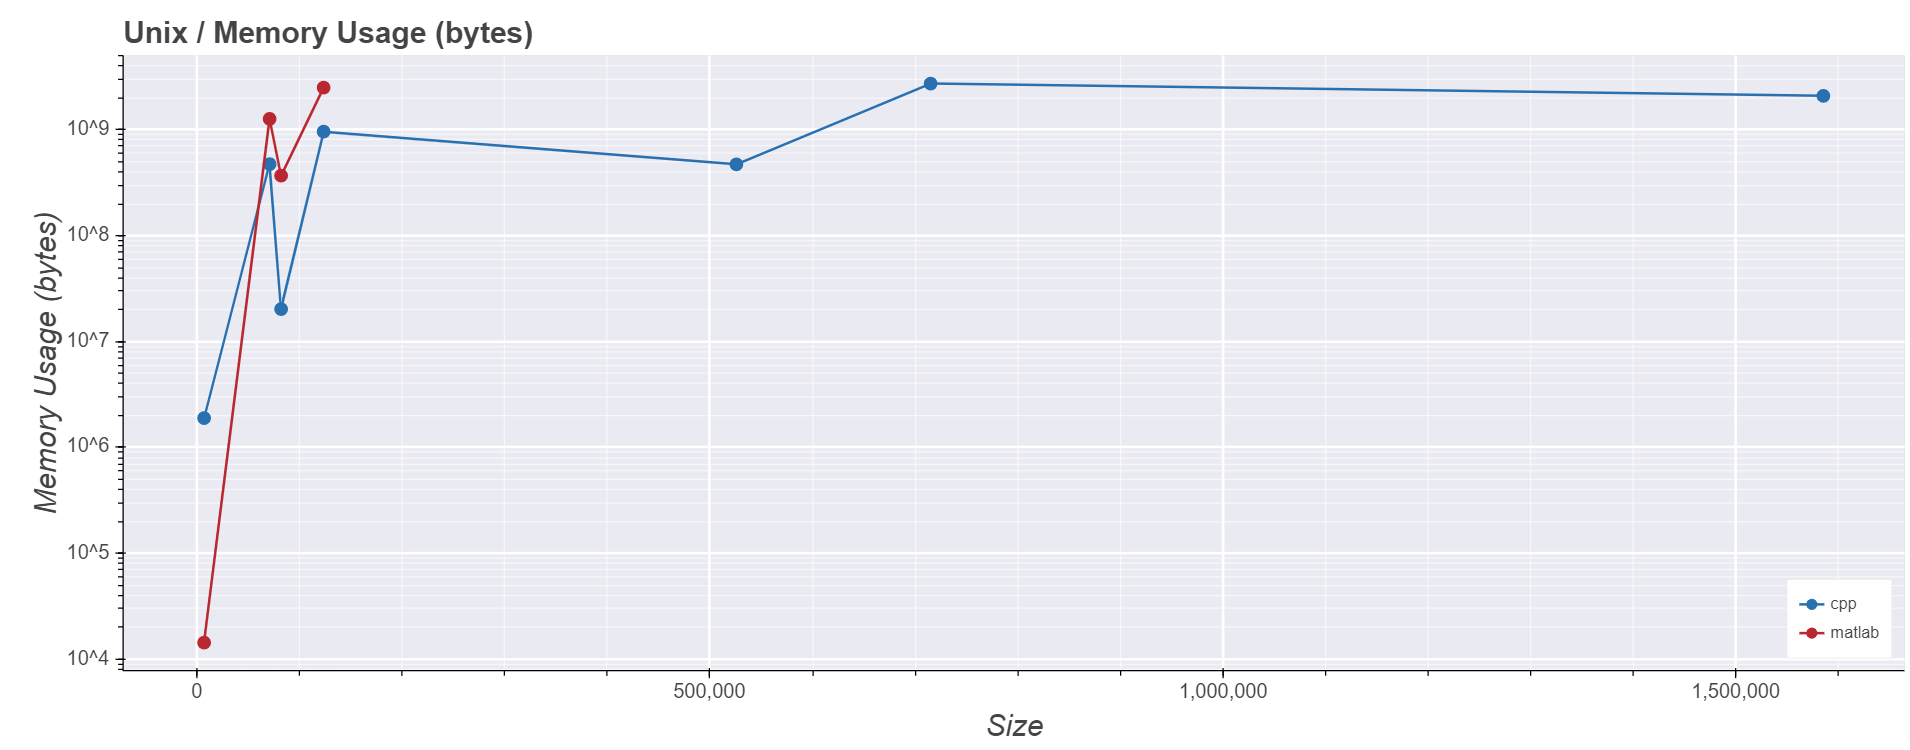
\includegraphics[width=1.4\linewidth]{unix_memory.png}}
\end{figure}

\section{Conclusioni}
\section{Code}

\end{document}